%% Submissions for peer-review must enable line-numbering
%% using the lineno option in the \documentclass command.
%%
%% Preprints and camera-ready submissions do not need
%% line numbers, and should have this option removed.
%%
%% Please note that the line numbering option requires
%% version 1.1 or newer of the wlpeerj.cls file.
\def\tightlist{}

\documentclass[fleqn,10pt,lineno]{wlpeerj} % for journal submissions
% \documentclass[fleqn,10pt]{wlpeerj} % for preprint submissions

\usepackage{longtable}
\usepackage{hyperref}
\PassOptionsToPackage{hyphens}{url}\usepackage{hyperref}
%\usepackage[hyphens]{url}

\title{The Effect of Tides on Nearshore Environmental DNA}

\author{Ryan P. Kelly}
\author{Ram\'{o}n Gallego}
\author{Emily Jacobs-Palmer}
\affil{University of Washington, School of Marine and Environmental Affairs, Seattle, Washington USA}
%\affil[1]%{Address of second author}
\corrauthor{Ram\'{o}n Gallego}{rgallego@uw.edu}

%\keywords{Open access, open access journal, scholarly publishing, publication fees, article processing charges, science policy}

\begin{abstract}
Organisms of all kinds leave genetic traces in their environments, and in recent years, sequencing this environmental DNA (eDNA) has become a tractable means of surveying many species using water, air, or soil samples. The technique is beginning to become a core tool for ecologists, environmental scientists, and biologists of many kinds, but the temporal resolution of eDNA sampling is often unclear, limiting the ecological interpretations of the resulting datasets. Here, in a temporally and spatially replicated field study using ca. 330bp of COI mtDNA as a marker, we find that nearshore organismal communities as detected by eDNA are largely consistent across tides. Our findings suggest that nearshore eDNA tends to be endogenous to the site and water mass sampled, rather changing systematically as waters change over during the tidal cycle. However, where entire water masses change, we find that the eDNA communities change in concert, again suggesting a close association between the habitat sampled and the eDNA community recovered. 
\end{abstract}

\begin{document}

\flushbottom
\maketitle
\thispagestyle{empty}

\section{Introduction}\label{introduction}

As environmental DNA (eDNA) becomes an increasingly important tool in
ecological research (Sigsgaard et al. 2016,Deiner et al. (2017)), it is
critical to understand how techniques for eDNA collection and analysis
perform under real-world conditions (Jesse A. Port et al. 2016). In
particular, we must characterize the spatial and temporal resolution of
amplicon-sequencing studies in order to confidently detect ecological
patterns in the field (O'Donnell et al. 2017); like any sampling
technique, eDNA can reveal the effects of a phenomenon only where
variation due to the phenomenon being studied is sufficiently large that
it is detectable relative to background variation (e.g., among
replicates or time points).

Most efforts to quantify the behavior of eDNA in the field have taken
the form of quantitative PCR (qPCR) studies, in which the concentration
of target template DNA -- either a particular target species or else a
synthesized template not otherwise occurring in nature -- is measured
over space or time. Notable recent examples include documenting
degradation of DNA over tens of meters in the flow of artificial streams
(Jerde et al. 2016), caging fish and measuring eDNA concentration at
intervals downstream (Jane et al. 2015), estimating eDNA production and
degradation over time in a static environment (Sassoubre et al. 2016),
and estimating production and decay rates of both caged and wild fish in
a field setting (Wilcox et al. 2016), among others (e.g., Deiner and
Altermatt 2014; Thomsen et al. 2012). Although the details vary by
setting and by molecular assay, even with quite sensitive qPCR assays
the distance from its source that eDNA can reliably be detected appears
to be small, on the order of 10 -- 1000m.

By contrast, less work has focused on the behavior of eDNA as reflected
in ecological amplicon-sequencing studies. Port and colleagues showed
that vertebrate eDNA communities could be distinguished at intervals of
60m (Jesse A Port et al. 2016) in nearshore marine waters, and
(O'Donnell et al. 2017) suggested a similar spatial scale (\textless{}
75m) pertained to a broader metazoan dataset. These were each
single-time-point snapshots of animal species in dynamic environments,
however, and especially in marine and aquatic environments in which
spatial and temporal scales are linked by bulk transport of water, fine
spatial resolution could be obliterated by water movement.

The changing tides of nearshore marine habitats are rigorous testing
grounds for eDNA surveys, featuring large-scale turnover of water every
few hours (Babson, Kawase, and MacCready (2006)). In addition, these
nearshore habitats are among the most physically dynamic and
biologically diverse on earth (REFS), such that eDNA as a survey
technique holds particular promise for better understanding the
thousands of species that may co-occur at a single location.

Given recent work suggesting that eDNA signals are predominantly highly
localized in space and time (REFS) -- although in some circumstances,
eDNA may travel some distance {[}Deiner{]} -- we asked whether marine
eDNA community composition changes over tidal cycles at a given
location. A scenario in which eDNA communities change in unpredictable
ways with each new tide would suggest an exogeneous origin for that DNA,
such that DNA arrives at a site with incoming tides, drawn from a pool
of organisms existing elsewhere. By contrast, consistent eDNA
communities over multiple tidal cycles would strongly suggest an
endogenous origin and highly localized signal. An alternative scenario
is that high- and low-tide sigals at a site could differ in systematic
and consistent ways, reflecting either highly endogeneous DNA (i.e., the
species with which the water is in immediate contact at the time of
sampling) {[}or else perhaps exogeneous origin that varies predictably
with tide??{]}.

In a spatially- and temporarily-replicated study, we find that nearshore
COI eDNA community composition is not strongly influenced tide, and
instead remains largely consistent within each geographic location
across multiple successive tides. However, where dramatic shifts in the
physical and chemical environment suggest arrival of a new water mass at
a single sampling site, the eDNA community appears to change
accordingly. It therefore seems likely that changes in aqueous habitat
characteristics -- not tide itself -- yield changes in eukaryotic eDNA
communities.

\section{Methods}\label{methods}

\subsection{Field Sampling}\label{field-sampling}

\begin{figure}

{\centering 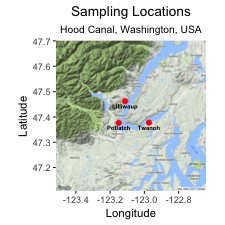
\includegraphics{figures/FIG1_sitemap-1} 

}

\caption{\label{fig:fig1}Nearshore sampling locations in Hood Canal, Washington, USA.}\label{fig:FIG1_sitemap}
\end{figure}

Our study design aimed to distinguish the effects of tide from
site-level community differences and from sampling error. Consequently,
we sampled each of three geographic locations (Fig 1; GPS coordinates
given in Suppl. Table 1) four times -- twice during an incoming tide,
and twice during an outgoing tide -- over a ca. 28-hour period. We
collected three 1-L water samples for eDNA analysis (ca. 10m apart) at
each site during each sampling event. Each sample was collected at the
surface (\textless{} 1m depth), using a ca. 3m-long pole with plastic
collection bottle attached. We kept samples on ice until they could be
processed, which occurred within hours of collection. We filtered 500mL
from each sample onto cellulose acetate filters (47mm diameter; 0.45um
pore size) under vacuum pressure, and preserved the filter at room
temperature in Longmire's buffer following Renshaw et al. (2015).
Deionized water served as a negative control for filtering. We measured
water temperature and salinity with a hand-held multiprobe (Hanna
Instruments, Inc. model XXXX), as well as measuring salinity with a
handheld manual refractometer; the latter instrument more reliably
reflected lab calibrations, and we use these measurements here.

\begin{longtable}[]{@{}lcc@{}}
\caption{Samples by site and tide, showing balanced sampling design.
Each site (N = 3) had a total of 4 sampling events (time points),
consisting of 3 water samples per event, and then 3-4 PCR replicates per
water sample, such that we sequenced 36-44 individual PCR replicates per
geographic sampling site. 35 of 36 samples were successfully processed,
with 93 individual replicates survived quality-control, described
below.}\tabularnewline
\toprule
& Incoming Tide & Outgoing Tide\tabularnewline
\midrule
\endfirsthead
\toprule
& Incoming Tide & Outgoing Tide\tabularnewline
\midrule
\endhead
Lilliwaup & 5 & 6\tabularnewline
Potlatch & 6 & 6\tabularnewline
Twanoh & 6 & 6\tabularnewline
\bottomrule
\end{longtable}

\subsection{DNA Extraction, Amplification, and
Sequencing}\label{dna-extraction-amplification-and-sequencing}

We extracted total DNA from the filters using a
phenol:chloroform:isoamyl alcohol protocol following ({\textbf{???}}),
resuspended the eluate in 200uL water, and used 1uL of diluted DNA
extract (1:10) as template for PCR. Although a single locus cannot
completely characterize the biodiversity at a particular location (see,
e.g., {\textbf{???}}), we used a 330bp fragment of COI to assess the
eukaryotic variance among our samples. This primer set ({\textbf{???}})
amplifies a broad array of taxa including representative diatoms,
dinoflagellates, metazoans, fungi, and others; here, we simply use this
primer set as an assay to characterize community similarity among
samples. We followed a two-step PCR protocol to first amplify and then
index our samples for sequencing, such that we could sequence many
samples on the same sequencing run while avoiding amplification bias due
to index sequence ({\textbf{???}}). PCR mixes were 1X HotStar Buffer,
2.5mM \(MgCl_2\), 0.5mM dNTP, 0.3\(\mu\)M of each primer and include 0.5
units of HotStar Taq (Qiagen Corp.) per 20 \(\mu\)L reaction. The first
round of PCR consisted of 40 cycles, including an annealing touchdown
from 62\(^\circ\)C to 46\(^\circ\)C (-1\(^\circ\)C per cycle), followed
by 25 cycles at 46\(^\circ\)C. The indexing PCR used a similar protocol
with only 10 cycles at 46\(^\circ\)C.

We generated three PCR replicates for each of 35 water samples (3
samples per sampling event, 4 sampling events per site, 3 sites = 36
water samples, of which 35 were processed successfully), and sequenced
each replicate individually in order to assess the variance in detected
eDNA communities due to stochasticity during amplification. We
simultaneously sequenced positive (Ostrich (\emph{Struthio camelus})
tissue, selected because of the absence of this species in our study
sites) controls with identical replication. We carried negative controls
through amplification, but did not sequence them, due to methodological
issues associated with library preparation in samples without any
discernable amplicon. No amplification was visible via gel
elecrophoresis in the negative controls, and fluorometry (Qubit; Thermo
Scientific) analysis showed negligible amounts of DNA present in those
samples after amplification. The positive controls provided us with
consistent estimates of cross-contamination (see below), which we used
in sequence quality-control prior to analysis.

Following library preparation according to manufacturers' protocols
(KAPA Biosystems, Wilmington, MA, USA; NEXTflex DNA barcodes, BIOO
Scientific, Austin, TX, USA), sequencing was carried out on an Illumina
MiSeq (250bp, paired-end) platform in two different batches: a MiSeq V.2
run and a MiSeq nano run. These were processed separately through the
first stages of bioinformatics analysis (see below), and then combined
after primer removal for dereplication. PCR replicates (derived from the
same sampled bottle of water) sequenced on different runs clustered
together without exception (see Results), and thus combining the data
from two sequencing runs was appropriate.

\subsection{Bioinformatics}\label{bioinformatics}

We processed the resulting sequence reads with a custom Unix-based
script ({\textbf{???}}), which calls third-party programs (Mahé et al.,
2015; Martin, 2011; Zhang et al., 2014) to move from raw sequence data
to a quality-controlled dataset of counts of sequences from operational
taxonomic units (OTUs). A total of 5,105,198 reads survived preliminary
quality-control in the bioinformatics pipeline, representing 149,829
OTUs, most of which were rare (\textless{} 5 reads). We controlled for
contamination in three ways, following our approach in ({\textbf{???}}).
First, to address the question of whether rare OTUs are a function of
low-level contamination or are true reflections of less-common
amplicons, we used a site-occupancy model to estimate the probability of
OTU occurrence (Royle and Link, 2006; Lahoz-Monfort et al. 2015), using
multiple PCR replicates of each environmental sample as independent
draws from a common binomial distribution. We eliminated from the
dataset any OTU with \textless{}80\% estimated probability of
occurrence, yielding a dataset of 4,811,014 reads (7,503 OTUs). We
retained the occupancy-probability data for each OTU for later use as an
alternative to simple presence-absence treatment of the final dataset
(see below). Second, we estimated (and then minimized) the effect of
potential cross-contamination among samples -- likely due to tag-jumping
{[}CITE{]} or similar effects -- as follows: (1) we calculated the
maximum proportional representation of each OTU across all control
(here, ostrich) samples, considering these to be estimates of the
proportional contribution of contamination to each OTU recovered from
the field samples. (2) We then subtracted this proportion from the
respective OTU in the field samples, yielding 4,370,486 reads (7,496
OTUs). Finally, we dropped samples that had highly dissimilar PCR
replicates (Bray-Curtis dissimilarities \textgreater{} 0.49, which were
outside of the 95\% confidence interval given the best-fit model of the
observed among-replicate dissimilarities). The result was a dataset of
4,164,517 reads (7,496 OTUs), or 81.57\% of the post-pipeline reads.

We rarefied read counts from each PCR replicate to allow for comparison
across water samples using the vegan package for R (Oksanen et al.,
2015). We carried out subsequent analyses on a single, illustrative
rarefaction draw; these did not vary substantially among the rarefaction
replicates (Supplemental Figure 1).

\subsection{Statistical Analysis}\label{statistical-analysis}

\subsubsection{Data Validation: Apportioning Variance in Bray-Curtis
Dissimilarity Among Sites, Sampling Events, Bottle Samples, and PCR
Replicates}\label{data-validation-apportioning-variance-in-bray-curtis-dissimilarity-among-sites-sampling-events-bottle-samples-and-pcr-replicates}

We calculated the variance in OTU communities at five hierarchical
levels -- between tides (incoming vs.~outgoing), among geographic sites
(N = 3), among sampling events within geographic sites (N = 4 per site),
among sample bottles within a sampling event (N = 3 per event per site),
and among PCR replicates (N = 3 per individual sample bottle; reflected
by the model residuals) -- using a PERMANOVA test on Bray-Curtis (OTU
count data) dissimilarity among sequenced replicates. Calculations were
carried out in R \cite{R_core} using the vegan \cite{} package. Having
established that the variance among PCR replicates and bottles was small
relative to variance among sampling events and geographic sites (see
Results), it was clear that our dataset had the necessary resolution to
detect community-level changes -- if any -- associated with changes in
tide.

\subsubsection{How Many Ecological Communities Are Present, and How
Similar are Communities Among Sites, Sampling Events, and
Tides?}\label{how-many-ecological-communities-are-present-and-how-similar-are-communities-among-sites-sampling-events-and-tides}

We then used Bray-Curtis dissimilarity to visualize differences among
sampled communities at each hierarchical level of organization, using
ordination (NMDS; R packages MASS \cite{} and ggplot2 \cite{}) and a
heatmap. Given the strong and consistent differentiation we identified
between two ecological communities in the eDNA data (see Results), we
then labeled these communities 1 and 2, and applied a set of standard
statistics to test for associations between community identity and
geographic site (Fisher's exact test), tidal direction (incoming
vs.~outgoing; chi-squared), and tidal height (logistic regression).

\subsubsection{Community Identity by Site and
Tide}\label{community-identity-by-site-and-tide}

We recovered tidal height data for our study sites during the relevant
dates from the National Oceanographic and Atmospheric Administration
data for Union, Washington (available at: \url{https://}
tidesandcurrents.noaa.gov/noaatidepredictions.html).

\subsubsection{Characterizing the Observed Ecological
Communities}\label{characterizing-the-observed-ecological-communities}

We stress that a single genetic locus provides only a biased and
incomplete view of an ecosystem (see \cite{Kelly_et_al_multilocus} for
discussion), and although our purpose was to test for the effect of
tidal fluctuations on detected eDNA communities -- which does not
require taxonomic annotation of the recovered OTUs -- we were
nevertheless interested in the membership of the ecological communities
we detected. Our locus of choice, COI, provided a broad view of
ecosystem with 23 phyla in 8 kingdoms represented (see Supplemental
Table 2 for summary table). Planktonic microalgae dominated the read
counts, with approximately 91\% of annotated reads mapped to taxa in the
groups Chlorophyta and Phaeophyceae.

We assigned a taxonomic name to each OTU sequence using blastn (Camacho
et al., 2009) on a local version of the full NCBI nucleotide database
(current as of August 2017), recovering up to 100 hits per query
sequence and reconciling conflicts among equally good matches using the
last common ancestor approach implemented in MEGAN 6.4 (Huson et al.,
2011). 93.08\% of OTUs could be annotated at some taxonomic level, with
over half (57.54\%) being annotated to the level of taxonomic Family or
lower.

We report an index of community-wide changes across sampling events
using the top 8 {[}??{]} most common taxonomic Families reporesented in
the dataset. We carried out a finer-grained analysis to identify the
OTUs driving the observed community shifts at Twanoh by first using a
cannonical correspondence analysis (CCA), constrained by community
identity (1 vs.~2, identified as described above via NMDS), then
filtering the CCA scores by read count, such that we plotted only OTUs
that strongly differentiated communities and occurred at least 1000
times in the dataset. We then show these by taxonomic annotation, for
intelligibility.

\section{Results}\label{results}

\subsection{Community-Level similarity among replicates, sites, etc:
Apportioning variance in Bray-Curtis
Dissimilarity}\label{community-level-similarity-among-replicates-sites-etc-apportioning-variance-in-bray-curtis-dissimilarity}

To evaluate the spatial and temporal turnover between eDNA communities,
we first apportioned the observed variation in COI Bray-Curtis
dissimilarities (calculated using OTU read counts) among tides (incoming
vs.~outgoing), sampling sites, sampling events within a site, biological
replicates (individual bottles of water taken during the same sampling
event), and technical replicates (PCR replicates from the same bottle of
water). Across the whole dataset, ecological communities at different
sampling sites (20-50km apart) account for the largest fraction of the
variance (0.43), and different sampling events within those sites
account for a similarly high proportion (0.31). In contrast, biological
replicates (N = 3 bottles of water per sampling event, taken ca. 10m
apart) account for a small fraction (0.07) of the variance, with
differences among tides accounting for the smallest fraction of the
variance in community dissimilarity (0.06). The remainder -- 0.13 -- is
largely due to differences among technical PCR replicates (N = 3 per
bottle of water), much of which derives from stochasticity in the
presence of rare OTUs (Supplemental Figure 1). The comparitively low
variance issuing from biological and technical replicates relative to
sampling events and sites affords the resolution necessary to further
examine questions of community composition across space and time.

\begin{figure}

{\centering 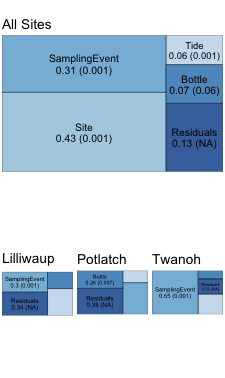
\includegraphics{figures/ADONIS_TreemapDiagrams-1} 

}

\caption{\label{fig:AdonisFigure}Results of PERMANOVA, apportioning variance by hierarchical levels of sampling design: Tide (incoming vs. outgoing), Sampling Site, Sampling Event (N = 4 time points per site), and Sampling Bottle (N = 3 bottles per sampling event). Residuals reflect variance among PCR replicates (N = 3 replicates per sampling bottle) as well as variation due to rarefaction stochasticity and other sampling effects. The upper panel reflects results for the dataset as a whole, with lower panels giving site-specific variances. Numbers reflect proportion of the variance explained by the indicated hierarchical level (R$^2$), with p-values in parentheses.}\label{fig:ADONIS_TreemapDiagrams}
\end{figure}

This approach to apportioning variance -- here, in Bray-Curtis
dissimilarity -- depends upon the total variance in the dataset being
analyzed. Analyzing individual site-level data eliminates the portion of
variance due to between-site differences, effectively amplifying the
contributions of the remaining hierarchical sampling levels. For each of
our three sampling sites, differences among sampling events were greater
than differences between tides (Figure 2). In these analysis, howevever,
we have treated tidal direction (incoming vs.~outgoing) as the highest
hierarchical level of our sampling design, effectively asking whether
eDNA assays reflected a coherent ``incoming'' tidal community and a
coherent ``outoging'' tidal community across all sites. We find little
evidence of such communities.

If instead we think of tidal turnovers, within a site, as a series of
events that each might influence community composition, we can measure
the buildup of Bray-Curtis dissimilarities over time and tide. Treating
our first sampling event at each site as the reference point for that
site, each sampling event occurred at a subsequent point in time and
after one or more changes in tide. If ecological communities within each
site remain consistent over time, we expect the Bray-Curtis values of
the community at time zero (the reference community) vs.~time one (the
subsequent sampling event) to be identical to the dissimilarity values
among bottles taken within the same sampling event.

\begin{figure}

{\centering 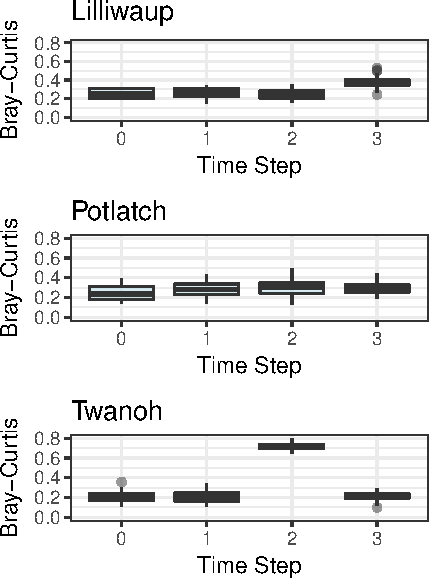
\includegraphics{figures/BrayCurtis_timeSeries-1} 

}

\caption{\label{fig:TimeSeriesFigure}Comparison of Bray-Curtis dissimilarities within a reference sampling event (Time step = 0) and between the reference sample and subsequent samples at the same site (Time Steps 1, 2, and 3). Subsequent time steps reflect the accumulation of ecological eDNA differences over hours as the tide moves in and out. Sites shown individually. Note the relatively small accumulation of Bray-Curtis dissimilarity across time and tides with the exception of the Twanoh event described elsewhere, which shifts the community significantly. Y-axes identical to facilitate comparison across sites.}\label{fig:BrayCurtis_timeSeries}
\end{figure}

We assessed each sampling site in this way (Figure 3), showing little
change in community dissimilarity as a function of tidal change (or
indeed of time). In all three sites, Bray-Curtis values remain stable
across multiple tide changes, with no continuously increasing trend over
time. Instead, two events stand out as statistically significant
(Kruskal-Wallis, p \textless{} 0.01): a moderate increase at Lilliwaup
at time step 3 (ca. 26 hours after the reference sample, from median
0.26 to 1), and a far larger jump in a single time point at Twanoh (ca.
19 hours after reference; from 0.2 to 0.72, before returning to its
reference value in the subsequent sampling event). Neither tidal
direction (incoming vs.~outgoing) nor individual tidal events therefore
consistently drive differences in sampled eDNA communities, but as
described below, individual changes in such as those seen in the Twanoh
changeover event, bear further scrutiny.

\section{How Many Ecological Communities Are
Present?}\label{how-many-ecological-communities-are-present}

\begin{figure}

{\centering 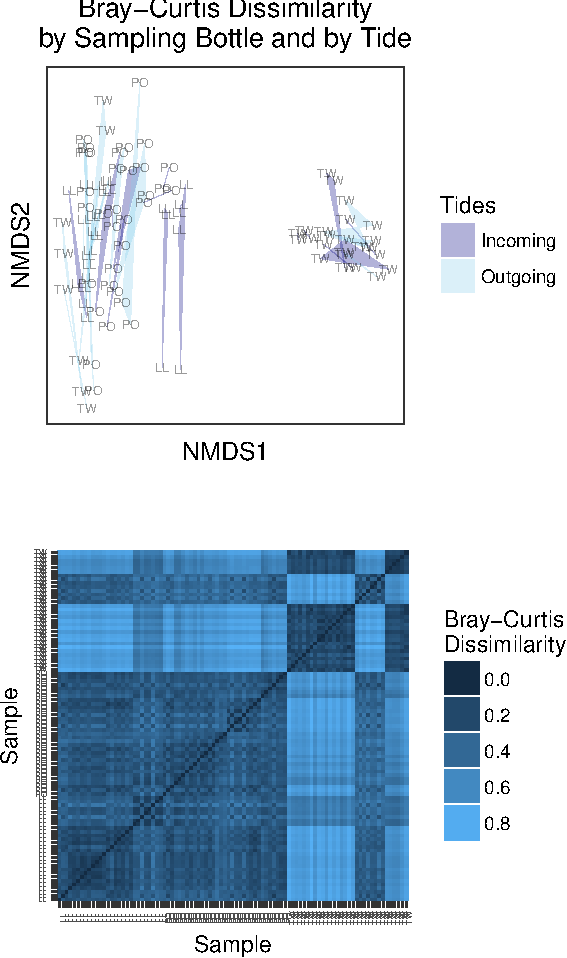
\includegraphics{figures/multiplot_NMDS_BottleTide-1} 

}

\caption{\label{fig:fig3}(A) Ordination plot (non-metric multidimensional scaling; NMDS) plot of Bray-Curtis dissimilarities among sequenced replicates, by sampling bottle (polygon) and tide (polygon color). (B) The same data shown as a heatmap, ordered by site identity. Only the Twanoh samples (upper right) stand out as having substantial heterogeneity, reflecting the two different communities present during different sampling events at that site. Site labels: TW = Twanoh, PO = Potlatch, LL = Lilliwaup.}\label{fig:multiplot_NMDS_BottleTide}
\end{figure}

An ordination plot of Bray-Curtis distances among each of our sequenced
replicates (Figure 3a) distinguishes two clusters of eDNA communities
present in the dataset. In agreement with the analysis of variance,
technical PCR replicates and biological replicates consistently cluster
closely in ordination space, yet two non-overlapping eDNA sequence
assemblages appear on this plot. A heatmap of the same Bray-Curtis
values reveals the underlying magnitudes of dissimilarity and
clustering, showing two clearly distinct communities of eDNA sequences
(Fig 3b). The two observed sequence clusters are primarily associated
with sampling site: the left-hand community (ordination plot; Fig 3a) is
present in all technical and environmental replicates of all Lilliwaup
and Potlatch samples, and in all such replicates from a single Twanoh
sampling event. By contrast, the right-hand community is only present in
the remaining three Twanoh samples.

\section{Community Identity by Site and
Tide}\label{community-identity-by-site-and-tide-1}

\begin{figure}

{\centering 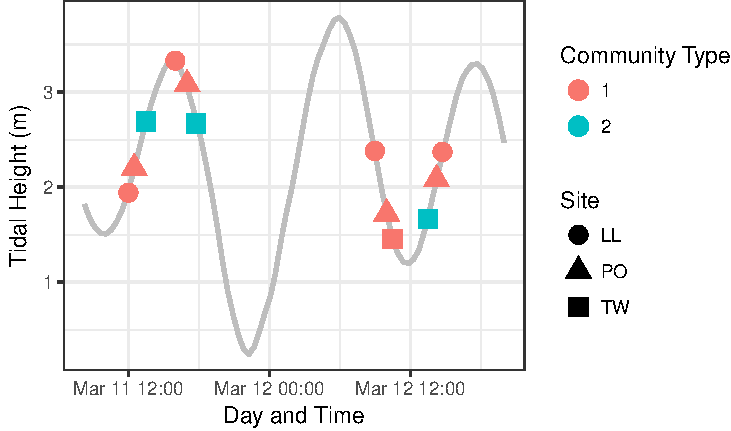
\includegraphics{figures/tide_community_figure-1} 

}

\caption{\label{fig:fig4}eDNA Communities by Time, Tide, and Site. We identify community type 1 as the dominant eDNA community (as seen in Figure 3, which appears at every geographic site), and community type 2 as the distinct type occurring only at Twanoh. See text for community descriptions.}\label{fig:tide_community_figure}
\end{figure}

To examine the relationship of each eDNA community with tide, we first
visually examined the mapping of tidal direction onto our ordination
analysis (Figure 3a; polygon color) and plotted community membership of
each sample across the tidal cycle during collection (Figure 4). Both
qualitatively indicate a lack of association between tidal direction or
height and the two eDNA communities. Quantitatively, by sampling event,
it is clear that community is independent of tidal height (p = 0.39;
linear regression) and of tidal direction (incoming vs.~outgoing; p =
0.163; \(\chi^2\)), but is related imperfectly to site identity (p =
1.554e-15; Fisher's exact test), as suggested previously (Figures 3a,
4). The single Twanoh sample belonging to eDNA Community 1 suggests that
geography does not fully explain differences between these communities,
and that ecological variables warrant further investigation as driving
differences in communities.

{[}insert ref to supplemental figure, time-series.{]}

\subsection{Environmental Co-variates Assocated with Community
Change}\label{environmental-co-variates-assocated-with-community-change}

To identify ecological factors that might distinguish the two eDNA
assemblages observed, we modeled the association of each sample's
temperature, salinity, DNA extraction concentration (which we speculate
is a proxy for primary productivity), and site identity with communities
1 and 2. Salinity and temperature explain nearly all of the variance in
community type (logistic regression best-fit model; null deviance =
84.79, residual deviance = 1.033e-09): we observe community 2 in fresher
(\textless{} 20ppt) and colder (\textless{} 9\(^\circ\)C) water than we
find community 1. Twanoh, in the southeastern portion of Hood Canal most
distant from the ocean, routinely experiences these kinds of fresher,
colder water events in our sampling month (March), unlike the main stem
of the Canal (Supplemental Figure).

In summary, the eDNA communities are more closely associated with
ecological variables -- salinity and temperature -- than with tide, or
even with geographical origin. This suggests that the two eDNA
assemblages may represent different aqueous habitat types, and led us to
investigate their taxonomic composition. We show the ecological and
biological context of each community sample in Figure X, before
highlighting the taxa that are particularly influential in defining the
two communities.

\section{Which organisms make up communities 1 and
2?}\label{which-organisms-make-up-communities-1-and-2}

\begin{figure}

{\centering 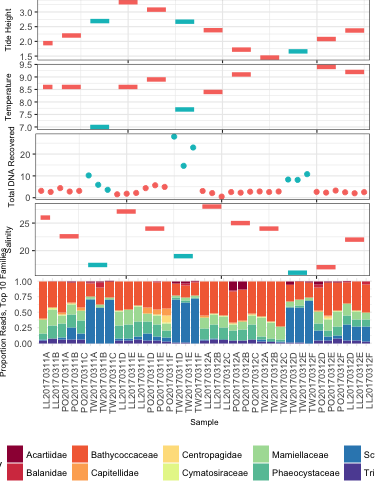
\includegraphics{figures/multiplot_community_membership-1} 

}

\caption{\label{fig:fig5}Tidal height (m), Water temperature (C), DNA concentration recovered (ng/mL), Salinity (ppt), and proportion of DNA reads allocated among the top 10 Families in the annotated dataset.}\label{fig:multiplot_community_membership}
\end{figure}

To identify the taxonomic groups that most strongly differentiate
ecological communities 1 and 2 at Twanoh, the location at which we
detected both communities at different points in time, we performed a
constrained canonical correspondence analysis (CCA) principal component
analysis on the OTU counts and filtered for highly discriminating OTUs
with high read counts (\textgreater{} 1000 reads). We then \ldots{}

To examine the turnover between ecological communities that occured in
the span of X hours at a single site (despite previous directional
shifts in tide at this location not resulting in a community
change-over) changing communities), we focused further on the community
composition of the two samples taken at Twanoh on March 12 at 11:00
(Community 1) and 13:00 (Community 2)\ldots{}

{[}, including Bathycoccus (green algae) and Micromonas (green algae),
Phaeocystis (green algae), Barantolla (polychaete worm with larval
phase), Balanus (barnacle with larval phase), Minutocellus (algae),
Centropages (copepod), Homo (terrestrial mammal), and Dictyocha
(photosynthetic algae) {]}

A handful of common green algae and benthic invertebrates (each of which
have larval phases) therefore distinguish the two communities we
identify with COI. However, given the well-known effects of primer bias
-- by which the apparent abundance of some taxa can be grossly distorted
by equating read count to organismal abundance -- we stress that here we
are using a single primer set as an index of community similarity,
rather than as an accurate reflection of the abundances of taxa present
in the water.

\begin{figure}

{\centering 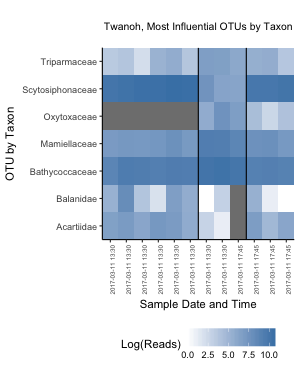
\includegraphics{figures/TW_Order_turnover-1} 

}

\caption{\label{fig:fig7}Most influential OTUs, plotted by taxonomic Order, distinguishing the two ecological communities observed in water samples from Twanoh State Park. Shown are the taxonomic Orders of OTUs with at least 1000 reads in the rarefied dataset, and having a constrained canonical correspondence analysis (CCA) score of greater than 0.7 (absolute value), which in our dataset most clearly divides the two communities. See text for CCA details. The vertical black lines in the chart delineate the communities identified previously by NMDS (see Figure 3a), with the time of each sample given along the x-axis, showing the shift from one community to the other -- and then largely back again -- within less than 24 hours. Note that each block of samples reflects a different point in the tidal cycle, and that the first two time points indicate a continuity of community membership despite a change in tide (see Figure 4).}\label{fig:TW_Order_turnover}
\end{figure}

\section{Discussion}\label{discussion}

Environmental DNA is rapidly becoming an essential and widely-used tool
to identify community membership in aquatic environments (review REFS).
It is not yet clear to what extent the sequences identified in eDNA
studies reflect the presence of local organisms in time and space,
however (locality REFS). Of particular interest in marine systems is the
influence of tide on the detection of ecological communities: Must
sampling schemes standardize tidal height and direction during
collection to detect consistent groups of species? Does each tide bring
with it a new water masse, carrying exogenous DNA, or do the sequences
detected at any given time accurately reflect the species present within
a habitat in that moment? To address these questions, we collected and
analyzed eDNA communities at three different sites along the Hood Canal
over the course of two tidal turnovers (Figure X - sampling scheme).
Thus, for each site, we were able to examine the influence of reversals
in tidal direction on two separate occasions.

When analyzed together, eDNA collections from three locations
(Lilliwaup, Potlatch, and Twanoh) show substantial variance in OTU
membership and prevalence associated primarily with geographic location
(Adonis table/fig). Grouping of samples in ordination space is also
strongly associated with site, rather than with tide (all-sample NMDS).
Together, these results suggest that eDNA surveys designed to clarify
relationships between distinct ecological communities are not likely to
suffer substantially from sample collection at varying points in the
tidal cycle, because the twice-daily exchange (or at least, mass
movement) of water into- and out of our sampling sites appeared to have
little influence on the sequences detected overall.

Although the effect of tide on eDNA community composition is small when
multiple geographic sites are considered simultaneously, tidal direction
may still strongly influence the OTUs detected within a single location.
The existence of among-site differences in ecological community in fact
provide the resolution necessary to detect such a local influence of
tide, if present - exogenous DNA arriving periodically with tidal flow
at each site might closely resemble neighboring communities, and differ
consistently from endogenous DNA collected on the ebb tide, which has
spent hours in contact with local benthic flora and fauna. A
site-by-site analysis reveals that a substantial proportion of the
variance in OTU counts is associated with tide, but never as much as is
associated with sampling event (Adonis single site table/figs).
Additionally, visualization of samples from each geographic location in
ordination space shows no recognizable grouping by tide (NMDS single
site figs). Finally, the eDNA community present at a single site tends
to drift over time, decreasing in similarity to the initial sample,
regardless of tide (Time graphs). Together, these results suggest that
the effect of tidal flow on eDNA community membership increases when
geographic sites are considered independently, but remains small in
comparison to the importance of sampling event, overall.

Rather than tide, ecological variables such as temperature and salinity,
each of which differ among sites and sampling events, seem to drive the
bulk of the variance in eDNA community membership (Stacked Figure).
These variables are key determinants of marine habitat type, especially
for planktonic species. At Twanoh we sampled by chance a dramatic
turnover in species composition within the span of just a few hours, and
a parallel shift in ecological variables. The families most notably
associated with this shift in community are indeed planktonic,
suggesting that eDNA survey methodology succeeded in identifying the
species physically present within the water column at the time of
sampling. However, the entrance and exit of a water masse and planktonic
community with characteristics more common at neighboring sites
decreased but did not eradicate the signal from sessile species that
consistently appeared at Twanoh. In summary, the sequenced eDNA
community reflects contributions from both organisms living within the
water itself, as well as sessile species in contact with that more
mobile community.

Taken together, our results suggest that eDNA samples taken from even
highly dynamic environments reflect recent contributions from local
species. With the exception of the occasional movement of water masses
representing distinct habitats for planktonic organisms, the eDNA
communities we sampled at three geographic sites were largely stable
over time and tide. Practically, this suggests that intertidal eDNA
research should be performed with substantial attention to ecological
variables such as temperature and salinity, which serve as markers of
the aqueous habitat present, and may not remain consistent
geographically. In contrast, tidal turnover appears to be a secondary
consideration that does not dramatically or consistently affect the
commmunity sampled, even within a single geographic location. Marine
intertidal eDNA surveys therefore appear to reflect the endogenous DNA
of the organisms present in the water and on the benthic substrate at
the time of sampling.

{[}eDNA sequenced from a nearshore habitat is likely a function of
(production by species in the water column) + (production by sessile,
infaunal, or otherwise locally present species) + (transport from
elsewhere) - (transport to elsewhere) - (degradation and sequestration).
Without modeling these terms explicitly, our results are consistent with
earlier findings that long-distance transport of eDNA appears unlikely:
each of our sites showed consistent differences, despite being located
within 10s of km of one another. Furthermore, the water changeover at
Twanoh sheds light on the balance between water- and surface-generated
eDNA\ldots{} {]}

{[}if we see Hood Canal as a large, homogeneous pool of DNA, sites
wouldn't sort. But they do. and sites remain stable over time,
relatively. so DNA isn't just associated with water, because water
characteristics are similar in most instances (it's the same water mass
at LL and PO, but the communities are predictably different). So there
must be a water-mass term and a non-water-mass term.{]}

\subsection{Acknowledgements}\label{acknowledgements}

We thank K. Cribari for lab assistance, as well as R. Morris, G. Rocap,
and V. Armbrust at the UW Center for Environmental Genomics. Special
thanks to M. Kelly, A. Ram'\{o\}n-Laca, and E. Flynn for facilitating
fieldwork, and Julieta, Damián, and Owen for field assistance. We are
also greatful to L. Park, J. O'Donnell, K. Nichols, and P. Schwenke at
NMFS for sequencing support and expertise.

\subsection{Funding}\label{funding}

This work was made possible by grant 2016-65101 from the David and
Lucile Packard Foundation to RPK.

\section{Supplemental Information}\label{supplemental-information}

\begin{table}

\caption{\label{tab:Supplement_GPScoordinatesSamplingAreas}Supplemental Table 1: Sampling Sites in Hood Canal, Washington, USA. Samples were taken intertidally, in water less than 1m deep.}
\centering
\begin{tabular}[t]{c|c|c}
\hline
Site & Latitude & Longitide\\
\hline
Lilliwaup State Park & 47.46 & -123.1\\
\hline
Potlatch State Park & 47.38 & -123.2\\
\hline
Twanoh State Park & 47.38 & -123.0\\
\hline
\end{tabular}
\end{table}

\begin{longtable}[]{@{}ccccccc@{}}
\caption{Summary of unique annotations, by taxonomic rank, in the COI
dataset.}\tabularnewline
\toprule
Kingdom & Phylum & Classes & Orders & Families & Genera &
OtherRank\tabularnewline
\midrule
\endfirsthead
\toprule
Kingdom & Phylum & Classes & Orders & Families & Genera &
OtherRank\tabularnewline
\midrule
\endhead
Bacteria & Proteobacteria & 4 & 4 & 2 & 0 & 0\tabularnewline
Diatoms & Bacillariophyta & 11 & 17 & 24 & 0 & 5\tabularnewline
Dinoflagellates & Dinoflagellata & 7 & 12 & 12 & 0 & 0\tabularnewline
Fungi & Ascomycota & 5 & 7 & 10 & 0 & 6\tabularnewline
Fungi & Basidiomycota & 2 & 3 & 3 & 0 & 2\tabularnewline
Fungi & Mucoromycota & 1 & 1 & 1 & 0 & 0\tabularnewline
Heterokonta & Phaeophyceae & 6 & 14 & 37 & 0 & 4\tabularnewline
Metazoa & Annelida & 5 & 9 & 12 & 0 & 4\tabularnewline
Metazoa & Arthropoda & 20 & 67 & 80 & 0 & 43\tabularnewline
Metazoa & Brachiopoda & 0 & 0 & 1 & 0 & 0\tabularnewline
Metazoa & Bryozoa & 1 & 1 & 1 & 0 & 0\tabularnewline
Metazoa & Chordata & 13 & 16 & 17 & 0 & 3\tabularnewline
Metazoa & Cnidaria & 5 & 13 & 18 & 0 & 4\tabularnewline
Metazoa & Echinodermata & 1 & 1 & 2 & 0 & 0\tabularnewline
Metazoa & Gastrotricha & 1 & 1 & 1 & 0 & 0\tabularnewline
Metazoa & Mollusca & 7 & 20 & 23 & 0 & 3\tabularnewline
Metazoa & Nematoda & 1 & 1 & 1 & 0 & 0\tabularnewline
Metazoa & Nemertea & 1 & 2 & 2 & 0 & 2\tabularnewline
Metazoa & Porifera & 7 & 7 & 7 & 0 & 1\tabularnewline
Metazoa & Rotifera & 1 & 1 & 1 & 0 & 1\tabularnewline
Rhodophyta & Rhodophyta & 5 & 13 & 15 & 0 & 0\tabularnewline
Viridiplantae & Chlorophyta & 5 & 7 & 11 & 0 & 3\tabularnewline
Viridiplantae & Streptophyta & 4 & 4 & 4 & 0 & 0\tabularnewline
\bottomrule
\end{longtable}

\begin{figure}

{\centering 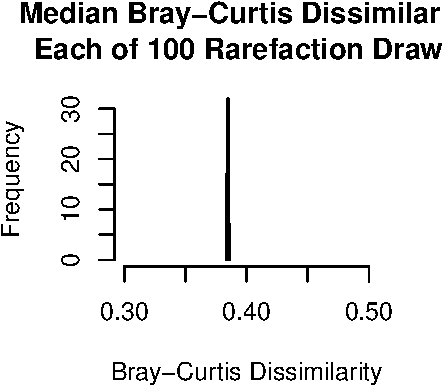
\includegraphics{figures/Load_Supplement_Rarefaction_data-1} 

}

\caption{\label{fig:SuppFig1} Differences among rarefaction draws expressed as median Bray-Curtis dissimilarities. The lack of variation in median dissimilarity among rarefaction draws underscores the fact that the results we present in the main manuscript do not differ substantially among different rarefaction draws.}\label{fig:Load_Supplement_Rarefaction_data}
\end{figure}

\begin{figure}

{\centering 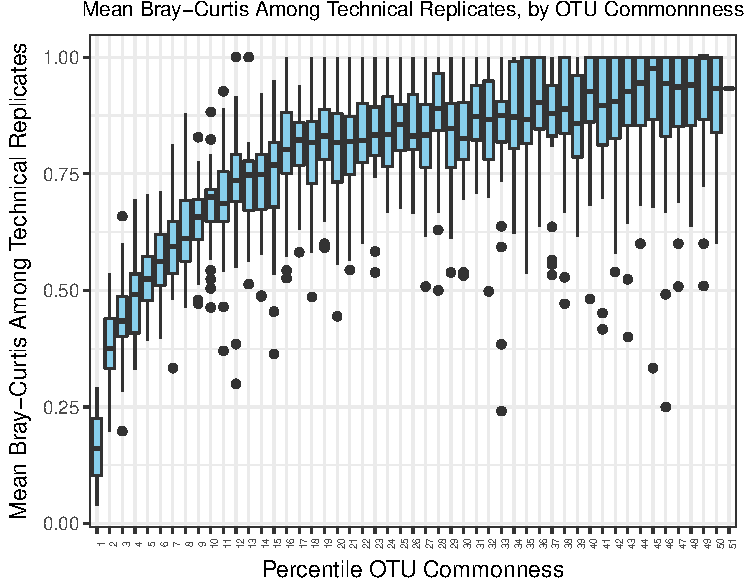
\includegraphics{20171117_Tides_and_eDNA_RPK_files/figure-latex/stochastic_variation_rareTail-1} 

}

\caption{\label{fig:SuppFig2}Variation among technical (PCR) replicates, expressed as Bray-Curtis dissimilarity among replicates using data subsets according to OTU commonness. Replicates are similar with respect to common OTUs, but stochasticity quickly dominates as OTUs become rarer, such that PCR replicates appear quite different with respect to OTUs in the bottom 90 percent of commonness.}\label{fig:stochastic_variation_rareTail}
\end{figure}

\begin{figure}

{\centering 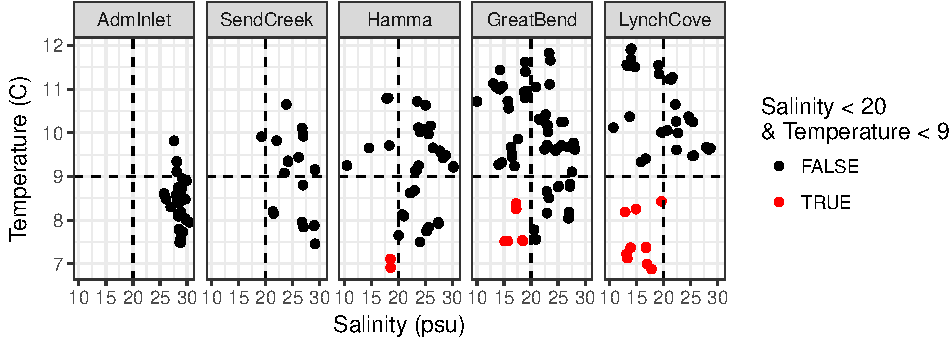
\includegraphics{20171117_Tides_and_eDNA_RPK_files/figure-latex/ContextualWaterData_WAEcology-1} 

}

\caption{\label{fig:SupplementalWaterChem}Contextual water data for the month of March from the Washington State Department of Ecology (https://fortress.wa.gov/ecy/eap/marinewq/mwdataset.asp). Plots are arranged north to south, with the southernmost point being Lynch Cove, near our sampled site of Twanoh. Red points indicate Temperature/Salinity data in the range of those in which we observed eDNA Community 2; these are far more common in the southern end of Hood Canal than in the north, which has a stronger oceanic influence.}\label{fig:ContextualWaterData_WAEcology}
\end{figure}\begin{table}

\caption{\label{tab:ContextualWaterData_WAEcology}Coordinates for WA Department of Ecology water quality sampling sites, which encompass the waters we sampled for the study presented in the main text.}
\centering
\begin{tabular}[t]{c|c|c}
\hline
Site Name & Latitude & Longitude\\
\hline
Admiralty Inlet & 48.03 & -122.6167\\
\hline
Send Creek & 47.667 & -122.82\\
\hline
Hamma Hamma & 47.5383 & -123.0083\\
\hline
Great Bend & 47.3567 & -123.0233\\
\hline
Lynch Cove & 47.3983 & -122.9283\\
\hline
\end{tabular}
\end{table}

Supplemental Figure X shows more southern points in the Hood Canal as
having an increased likelihood of cold, fresh water in March (red
points). These make up the following proportions: Admiralty Inlet = 0,
Send Creek = 0, Hamma Hamma = 0.05, Great Bend = 0.11, Lynch Cove =
0.28.

\section*{References}\label{references}
\addcontentsline{toc}{section}{References}

\hypertarget{refs}{}
\hypertarget{ref-Babson2006}{}
Babson, A. L., M. Kawase, and P. MacCready. 2006. ``Seasonal and
Interannual Variability in the Circulation of Puget Sound, Washington: A
Box Model Study.'' \emph{Atmosphere-Ocean} 44 (1). Taylor \& Francis:
29--45. doi:\href{https://doi.org/10.3137/ao.440103}{10.3137/ao.440103}.

\hypertarget{ref-deiner_transport_2014-1}{}
Deiner, Kristy, and Florian Altermatt. 2014. ``Transport Distance of
Invertebrate Environmental DNA in a Natural River.'' \emph{PLoS One} 9
(2): e88786.
doi:\href{https://doi.org/10.1371/journal.pone.0088786}{10.1371/journal.pone.0088786}.

\hypertarget{ref-deiner2017environmental}{}
Deiner, Kristy, Holly M Bik, Elvira Mächler, Mathew Seymour, Anaïs
Lacoursière-Roussel, Florian Altermatt, Simon Creer, et al. 2017.
``Environmental Dna Metabarcoding: Transforming How We Survey Animal and
Plant Communities.'' \emph{Molecular Ecology}. Wiley Online Library.

\hypertarget{ref-jane2015distance}{}
Jane, Stephen F, Taylor M Wilcox, Kevin S McKelvey, Michael K Young,
Michael K Schwartz, Winsor H Lowe, Benjamin H Letcher, and Andrew R
Whiteley. 2015. ``Distance, Flow and Pcr Inhibition: EDNA Dynamics in
Two Headwater Streams.'' \emph{Molecular Ecology Resources} 15 (1).
Wiley Online Library: 216--27.

\hypertarget{ref-jerde2016influence}{}
Jerde, Christopher L, Brett P Olds, Arial J Shogren, Elizabeth A
Andruszkiewicz, Andrew R Mahon, Diogo Bolster, and Jennifer L Tank.
2016. ``Influence of Stream Bottom Substrate on Retention and Transport
of Vertebrate Environmental Dna.'' \emph{Environmental Science \&
Technology} 50 (16). ACS Publications: 8770--9.

\hypertarget{ref-o2017spatial}{}
O'Donnell, James L, Ryan P Kelly, Andrew Olaf Shelton, Jameal F
Samhouri, Natalie C Lowell, and Gregory D Williams. 2017. ``Spatial
Distribution of Environmental Dna in a Nearshore Marine Habitat.''
\emph{PeerJ} 5. PeerJ Inc.: e3044.

\hypertarget{ref-port2016assessing}{}
Port, Jesse A, James L O'Donnell, Ofelia C Romero-Maraccini, Paul R
Leary, Steven Y Litvin, Kerry J Nickols, Kevan M Yamahara, and Ryan P
Kelly. 2016. ``Assessing Vertebrate Biodiversity in a Kelp Forest
Ecosystem Using Environmental Dna.'' \emph{Molecular Ecology} 25 (2).
Wiley Online Library: 527--41.

\hypertarget{ref-MEC:MEC13481}{}
Port, Jesse A., James L. O'Donnell, Ofelia C. Romero-Maraccini, Paul R.
Leary, Steven Y. Litvin, Kerry J. Nickols, Kevan M. Yamahara, and Ryan
P. Kelly. 2016. ``Assessing Vertebrate Biodiversity in a Kelp Forest
Ecosystem Using Environmental Dna.'' \emph{Molecular Ecology} 25 (2):
527--41.
doi:\href{https://doi.org/10.1111/mec.13481}{10.1111/mec.13481}.

\hypertarget{ref-sassoubre2016quantification}{}
Sassoubre, Lauren M, Kevan M Yamahara, Luke D Gardner, Barbara A Block,
and Alexandria B Boehm. 2016. ``Quantification of Environmental Dna
(EDNA) Shedding and Decay Rates for Three Marine Fish.''
\emph{Environmental Science \& Technology} 50 (19). ACS Publications:
10456--64.

\hypertarget{ref-sigsgaard2016population}{}
Sigsgaard, Eva Egelyng, Ida Broman Nielsen, Steffen Sanvig Bach, Eline D
Lorenzen, David Philip Robinson, Steen Wilhelm Knudsen, Mikkel Winther
Pedersen, et al. 2016. ``Population Characteristics of a Large Whale
Shark Aggregation Inferred from Seawater Environmental Dna.''
\emph{Nature Ecology \& Evolution} 1. Nature Publishing Group: 0004.

\hypertarget{ref-thomsen_detection_2012}{}
Thomsen, Philip Francis, Jos Kielgast, Lars Lønsmann Iversen, Peter Rask
Møller, Morten Rasmussen, and Eske Willerslev. 2012. ``Detection of a
Diverse Marine Fish Fauna Using Environmental DNA from Seawater
Samples.'' \emph{PloS One} 7 (8): e41732.
\url{http://dx.plos.org/10.1371/journal.pone.0041732.g003}.

\hypertarget{ref-wilcox2016understanding}{}
Wilcox, Taylor M, Kevin S McKelvey, Michael K Young, Adam J Sepulveda,
Bradley B Shepard, Stephen F Jane, Andrew R Whiteley, Winsor H Lowe, and
Michael K Schwartz. 2016. ``Understanding Environmental Dna Detection
Probabilities: A Case Study Using a Stream-Dwelling Char Salvelinus
Fontinalis.'' \emph{Biological Conservation} 194. Elsevier: 209--16.

\end{document}